\documentclass[12pt,a4paper]{article}

\usepackage[utf8]{inputenc}
\usepackage[english]{babel}
\usepackage{a4wide}
\usepackage{index}
\usepackage{blindtext}
\usepackage[graf, intHoriz, sinLU, showDirectores]{../assets/caratula}

\usepackage{amsmath}
\usepackage{amssymb}
\usepackage{bm}
\usepackage{hyperref}

\usepackage{adjustbox}
\usepackage{multirow}
\usepackage{array}
\usepackage{makecell}
\usepackage{subfig}

% chess typesetting
\usepackage{skak}
\usepackage{xskak}
\usepackage{wasysym} % other symbols

\usepackage{csquotes}
\usepackage[backend=biber]{biblatex}
\addbibresource{../refs.bib}

\integrante{Martín Emiliano Lombardo}{}{mlombardo9@gmail.com}
\titulo{Análisis de feature sets con redes neuronales NNUE para engines de ajedrez}
\fecha{\today}
\materia{}
\director{Agustín Sansone}{agustinsansone7@gmail.com}
\director{Diego Fernández Slezak}{dfslezak@dc.uba.ar}

\makeindex

\begin{document}

\maketitle

\tableofcontents
\newpage


\section{Introducción}

\begin{frame}
\frametitle{Ajedrez}
\begin{columns}
    \begin{column}{0.35\textwidth}
        \begin{itemize}
            \item Dos jugadores
            \item Suma cero
        \end{itemize}
    \end{column}
    \begin{column}{0.62\textwidth}
        \newchessgame
        \chessboard[showmover=false]
    \end{column}
\end{columns}
\end{frame}

\begin{frame}
\frametitle{Humano vs. Computadora}
\begin{columns}
    \begin{column}{0.2\textwidth}
        \newchessgame
        \chessboard[showmover=false,boardfontsize=10pt,hlabel=false,vlabel=false]
    \end{column}
    \begin{column}{0.8\textwidth}
        \begin{figure}
            \centering
            \visible<2->{\subfloat{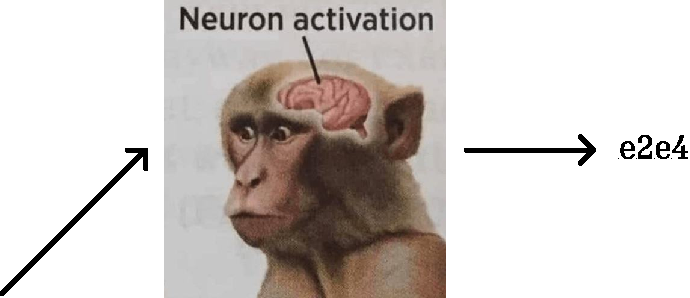
\includegraphics[width=0.8\linewidth]{../assets/slides/human.pdf}}}

            \visible<3->{\subfloat{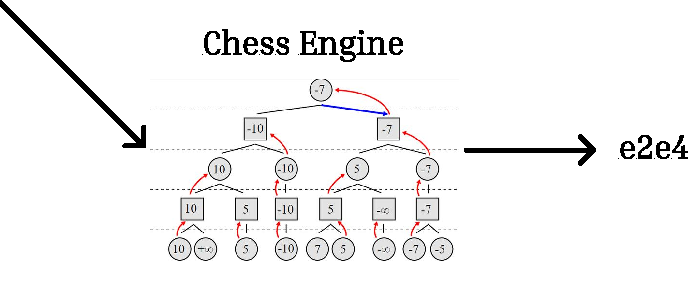
\includegraphics[width=0.8\linewidth]{../assets/slides/computer.pdf}}}
        \end{figure}
    \end{column}
\end{columns}
\end{frame}

\begin{frame}
\frametitle{Ajedrez como árbol}
\begin{figure}
    \centering
    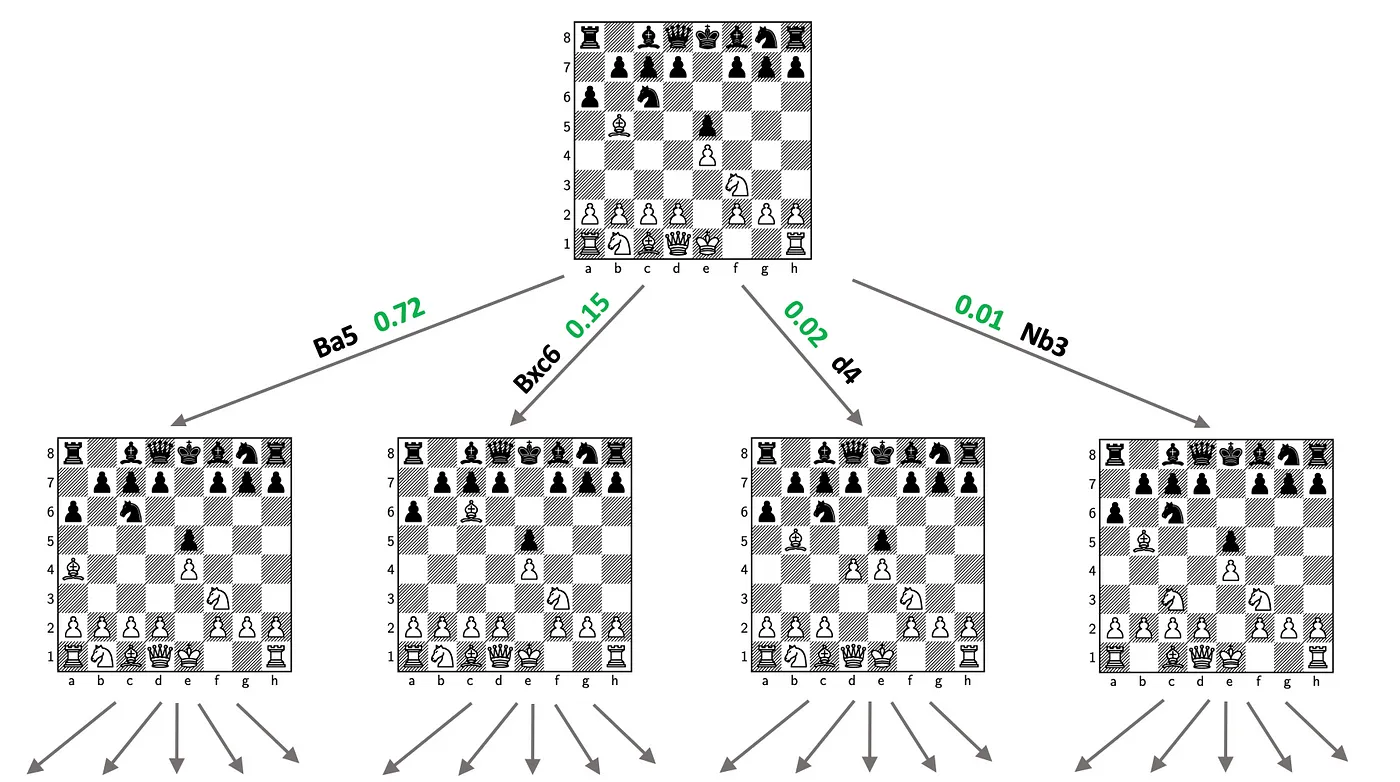
\includegraphics[width=1.0\linewidth]{../assets/slides/chess_tree.png}
\end{figure}
\end{frame}

\begin{frame}
\frametitle{Motores de ajedrez (Chess Engines)}
\begin{columns}
    \begin{column}{0.5\textwidth}
        \begin{itemize}
            \item<1-> Exploran el árbol de juego (Minimax, MCTS, etc.)
            \item<2-> Utilizan funciones de evaluación en las hojas
            \item<3-> La evaluación se propaga hacia arriba, según el algoritmo
        \end{itemize}
    \end{column}
    \begin{column}{0.6\textwidth}
        \begin{figure}
            \centering
            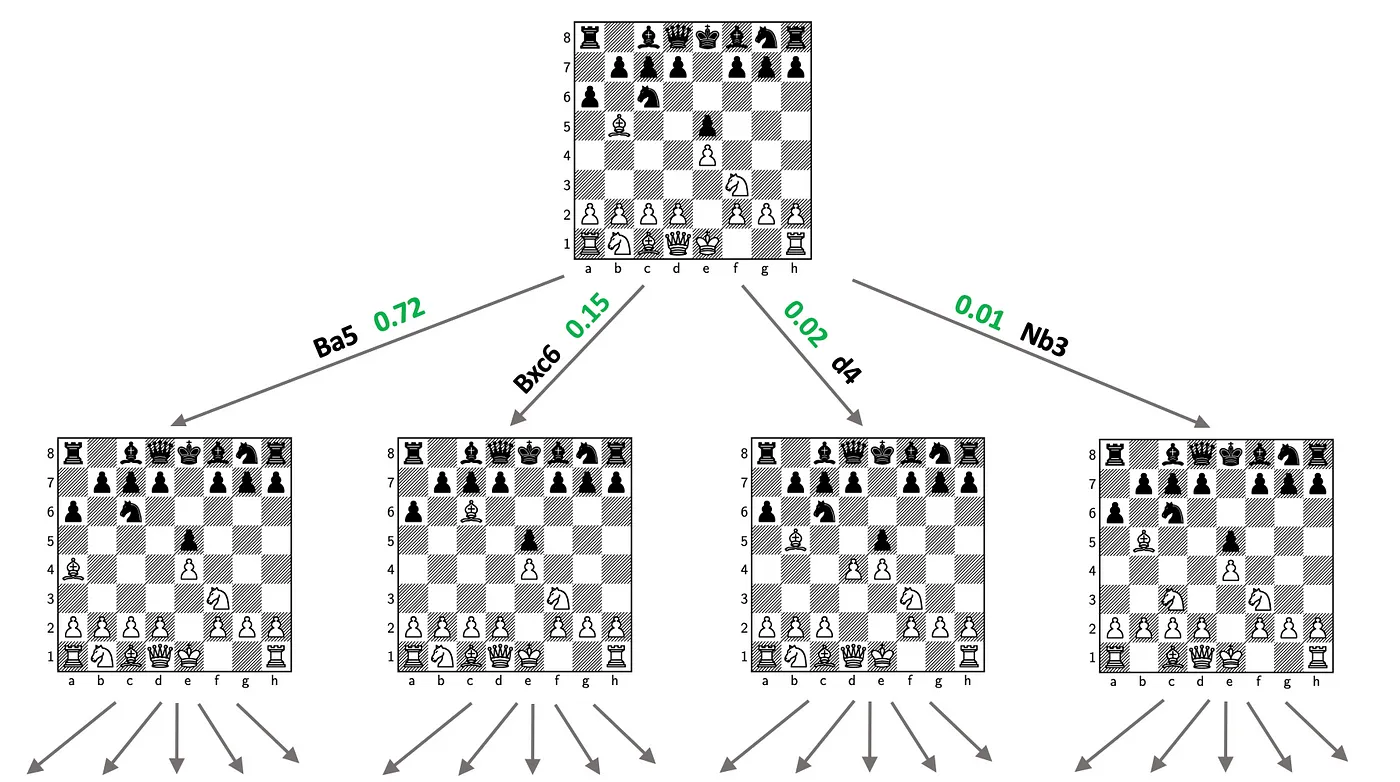
\includegraphics[width=0.9\linewidth]{../assets/slides/chess_tree.png}
        \end{figure}
    \end{column}
\end{columns}
\end{frame}

\begin{frame}
\frametitle{Función de evaluación o \enquote{eval}}
\begin{figure}
    \centering
    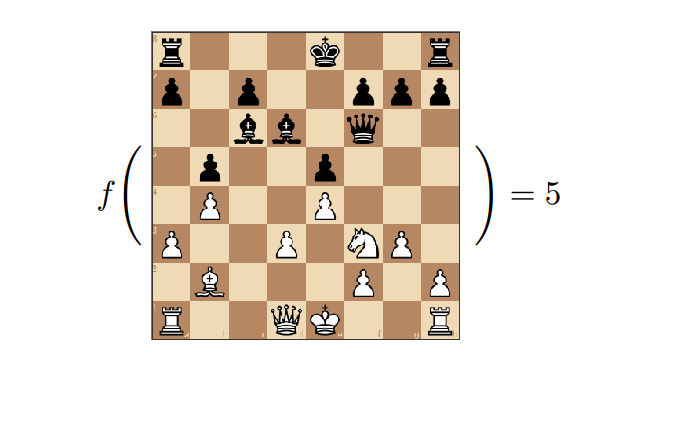
\includegraphics[width=0.8\linewidth]{../assets/slides/eval.png}
\end{figure}
\begin{center}
Intentan resumir todo el subárbol en un solo número. \\
En general son creadas \textit{artesanalmente}
\end{center}
\end{frame}

\begin{frame}
\frametitle{(adelanto) Feature sets: ¿Cómo transformar la posición a un vector para usar NNs?}
\begin{figure}
\centering
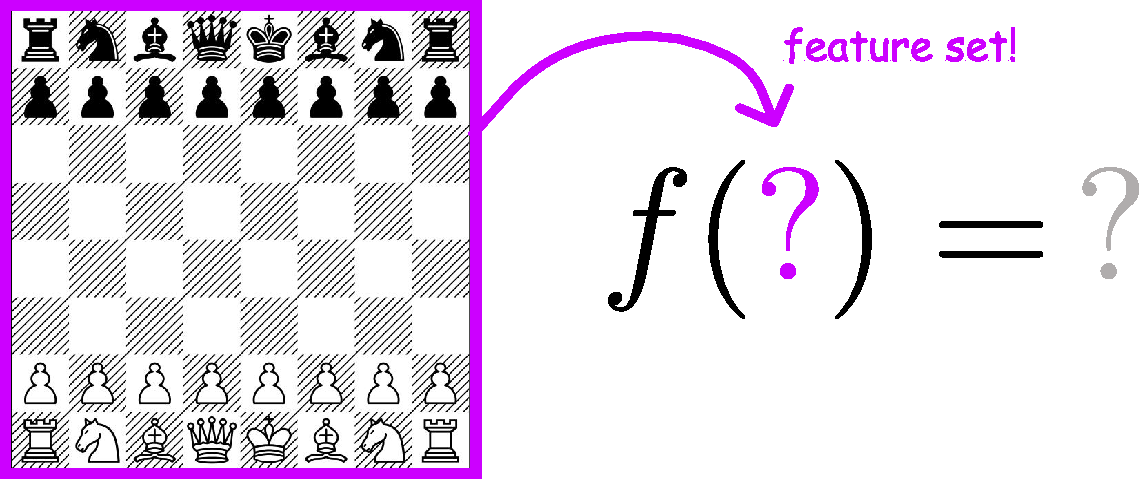
\includegraphics[width=1.0\linewidth]{../assets/slides/fs_motiv2.pdf}
\end{figure}
\end{frame}

\begin{frame}
\frametitle{Motores de ajedrez (breve historia)}
\begin{itemize}
    \item<1-> \textbf{1950s}: Se desarrollan los primeros \textit{algoritmos} de ajedrez
    \item<2-> \textbf{1960s+}: Aparecen los primeros \textit{motores de ajedrez}, lentos y débiles
    \item<3-> \textbf{1997} (hito): IBM DeepMind vence a Garry Kasparov en un torneo (superhuman)
    \item<4-> \textbf{2017 y 2018}: Google DeepMind publica AlphaGo Zero y su sucesor AlphaZero
    \begin{itemize}
        \item se reemplaza la función de evaluación por una red neuronal
    \end{itemize}
    \item<5-> \textbf{2018}: Yu Nasu introduce las redes \reflectbox{NNUE} para Shogi
    \item<6-> \textbf{2020}: Stockfish 12 introduce redes \reflectbox{NNUE} en su evaluación
    \begin{itemize}
        \item se utilizan a la par de evaluaciones artesanales
    \end{itemize}
    \item<7-> \textbf{2024}: Stockfish 16.1 elimina todo aspecto humano de su evaluación, todo es mediante redes neuronales
\end{itemize}
\end{frame}

\begin{frame}
\frametitle{Plan de la tesis}
El objetivo principal es \textbf{proponer y evaluar novedosos feature sets}. \pause Además, \textbf{probar una técnica de entrenamiento} no convencional. \\
\pause
\vspace{1em}
El plan de la presentación es el siguiente:
\begin{itemize}
\item<3-> Implementación de un motor de ajedrez clásico
\item<4-> Definición y ejemplos de feature sets
\item<5-> Introducción a las redes \reflectbox{NNUE}
\item<6-> Entrenamiento de las redes \reflectbox{NNUE}
\item<7-> Experimentos
\end{itemize}
\end{frame}

% \begin{frame}{Contenido}
% \tableofcontents
% \end{frame}

\newcommand{\white}{\fullmoon}
\newcommand{\black}{\newmoon}

\newcommand{\bigtimes}{\mathop{\raisebox{-0.5ex}{\scalebox{2}{$\times$}}}}

% https://texdoc.org/serve/chessboard/0
\newcounter{pieceindex}
\newcommand{\pieceBoard}{
    \newcount\pieceindex
    \setcounter{pieceindex}{0}
    \raisebox{-7ex}{
        \centering
        \chessboard[
            tinyboard,
            showmover=false,
            margin=false,
            padding=false,
            hlabel=false,
            vlabel=false,
            pgfstyle={text},
            %text=\fontsize{1.2ex}{1.2ex}\bfseries\sffamily \thepieceindex \stepcounter{pieceindex}, %  \currentwq
            text=\fontsize{1.2ex}{1.2ex}\bfseries\sffamily \currentwq,
            markboard
        ]
    }
}
\newcommand{\pieceRolesTable}{
    \begin{tabular}{|l|}
        \hline
        \sympawn\ Pawn \\
        \hline
        \symknight\ Knight \\
        \hline
        \symbishop\ Bishop \\
        \hline
        \symrook\ Rook \\
        \hline
        \symqueen\ Queen \\
        \hline
        \symking\ King \\
        \hline
    \end{tabular}
}
\newcommand{\pieceColorsTable}{
    \begin{tabular}{|l|}
        \hline
        $\white$ White \\
        \hline
        $\black$ Black \\
        \hline
    \end{tabular}
}

\newcommand{\fs}[1]{\textsc{#1}}


\section{Feature set (board encoding)}

To evaluate chess positions, we will use a neural network with an architecture explained in detail in the next chapter. In this chapter, we will build the one-dimensional input vector for such network, which can be described entirely by a feature set.

A feature set is a set built by a cartesian product of smaller sets of features, where each set extracts a different aspect of a position. Each tuple in the feature set corresponds to an element in the input vector, which will be set to $1$ if the aspects captured by the tuple is present in the position, and $0$ otherwise. If a tuple is present in a position, we say that the tuple is \textit{active}.

Let's consider some basic sets of features. The following sets encode positional information about the board:

\begin{center}
\begin{tabular}{cc}

$\begin{aligned}[t]
\fs{File} &= \{a, b, ..., h\} \\
\fs{Rank} &= \{1, 2, ..., 8\} \\
\fs{Square} &= \{a1, a2, ..., h8\}
\end{aligned}$

&

\raisebox{-10ex}{
\chessboard[
    tinyboard,
    showmover=false,
    pgfstyle={text},
    %text=\fontsize{1.2ex}{1.2ex}\bfseries\sffamily \thepieceindex \stepcounter{pieceindex}, %  \currentwq
    text=\fontsize{1.2ex}{1.2ex}\bfseries\sffamily \currentwq,
    markboard
]
}

\end{tabular}
\end{center}

And the following encode information about the pieces:

\begin{center}
$\begin{aligned}[t]
\fs{Role} &= \text{\{
    \sympawn\ Pawn,
    \symknight\ Knight,
    \symbishop\ Bishop,
    \symrook\ Rook,
    \symqueen\ Queen,
    \symking\ King\}}\textsuperscript{1} \\
\fs{Color} &= \text{\{\white\ White, \black\ Black\}}
\end{aligned}$
\end{center}

Since each set has to capture some information from the position, it must be stated explicitly. For example, consider the feature set $\fs{File}_{P} \times \fs{Color}_{P}$ where $P$ is \textit{any} piece in the board, meaning that the tuples $(file, color)$ that will be active are the ones where there is at least one piece in $file$ with the color $color$ (disregarding any other kind of information, like the piece's role). Another possible feature set could be $\fs{File}_{P} \times \fs{Role}_{P}$, with a similar interpretation. An illustration of the active features of these two feature sets for the same board is shown in Figure \ref{fig:active_features}.

\begin{figure}[h]
\centering

\begin{tabular}{cc}
\raisebox{-7ex}{
\chessboard[
    tinyboard,
    showmover=false,
    hlabel=false,
    setwhite={kc3, nc2, pa2, Pd4},
    addblack={Kc8,bh7, pa7}
]
}

&

\begin{tabular}{|c|p{4cm}|p{4cm}|p{0cm}}
\cline{2-3}
\multicolumn{1}{c|}{} & \multicolumn{2}{c|}{\centering Feature set} \\
\cline{2-3}
\multicolumn{1}{c|}{} & \centering $\fs{File}_{P} \times \fs{Color}_{P}$ & \centering $\fs{File}_{P} \times \fs{Role}_{P}$ & \\
\cline{1-3}
Active features &
(a, \white), (a, \black), (c, \black), (c, \white), (d, \white), (h, \black) &
(a, \sympawn), (c, \symking), (c, \symknight), (d, \sympawn), (h, \symbishop) \\
\cline{1-3}
\end{tabular}

\end{tabular}

\caption{Active features of the feature sets $\fs{File}_{P} \times \fs{Color}_{P}$ and $\fs{File}_{P} \times \fs{Role}_{P}$ for the same board.}
\label{fig:active_features}
\end{figure}

\footnotetext[1]{The color of the pieces have no meaning in the definition. They are present for illustrative purposes.}

\subsection{Sum $\oplus$}

% what to talk about:
% we want the network to find patterns between the two sets
% some feature sets can be built merging the features of two or more sets

The sum of two feature sets $\fs{A}$ and $\fs{B}$, denoted by $\fs{A} \oplus \fs{B}$, is a new feature set comprised of the tuples of both sets $\fs{A}$ and $\fs{B}$. These tuples do not interfere with each other, even if they have the same basic elements (e.g. h, 8, \symrook, \black), they \textbf{must} have different interpretations.
For example, given the feature sets $\fs{File}_{W}$ where $W$ is any white piece in the board and $\fs{File}_{B}$ where $B$ is any black piece in the board, the feature set $\fs{File}_{W} \oplus \fs{File}_{B}$ will have the basic elements $\{a, b, ..., h\}$ for both white and black pieces, but each with a different interpretation.

The sum operator is useful when we want to let the network find patterns combining information between two sets of features.



\subsection{Indexing}

The input to the network is a one-dimensional vector, so we need a way to map the tuples in a feature set to the elements in the input vector. The correct index for a tuple is computed using the order of the sets in the cartesian product and the size of each set, like strides in a multi-dimensional array. For this to work, each element in a set $S$ must correspond to a number between $0$ and $|S| - 1$. For example, the feature set $A \times B \times C$ has $|A| \times |B| \times |C|$ elements, and the tuple $(a, b, c)$ is mapped to the element indexed at $a \times |B| \times |C| + b \times |C| + c$.

The same striding logic applies to feature sets built with the sum operator, recursively. [example?]

\subsection{Dead features}

[arreglar, lo movi]
For every position, role and color each piece could be, there is a feature. There are 16 tuples in the set that will never be active: (a8..h8, \sympawn, \white) and (a1..h1, \sympawn, \black) that correspond to the white pawns in the last rank and the black pawns in the first rank. This is because pawns promote to another piece when they reach the opponent side of the board. Effectively, these will be dead neurons in the network, but this way we can keep the indexing straightforward. Most feature sets will have dead features, and the same logic applies.


\subsection{Feature sets}

In this section, we will define the feature sets that will be used in the experiments. We will start with some of the most basic yet reasonable feature sets, then move to feature sets that are used by engines or were used in the past, and finally some that have not been tried, to the best of our knowledge.

\subsubsection{\mdseries\fs{Piece}}

This feature set is the most natural encoding for a chess position. There is a one-to-one mapping between pieces in the board and features:

\begin{center}
    $\fs{Piece} = \fs{Square}_{P} \times \fs{Role}_{P} \times \fs{Color}_{P}$ \\
    for every $P$ piece in the board \\
    ~\\
    $64*6*2=768$ features
\end{center}

\subsubsection{\mdseries\fs{Compact}}

This is a very compact feature set that still retains all the information of the board, meaning everything can be reconstructed by the neural network:

\begin{center}
    $\fs{Compact} = (\fs{File}_{P} \times \fs{Role}_{P} \times \fs{Color}_{P}) \oplus (\fs{Rank}_{P} \times \fs{Role}_{P} \times \fs{Color}_{P})$ \\
    for every $P$ piece in the board \\
    ~\\
    $2*(8*6*2)=192$ features
\end{center}

\subsubsection{\mdseries\fs{King-Piece}}

\begin{center}
    $\fs{King-Piece} = \fs{Square}_{K} \times \fs{Piece}_{P}$ \\
    where $K$ is the king to move and $P$ is every \textit{non-king} piece in the board \\
    ~\\
    $64*(64*5*2)=40960$ features
\end{center}

There are variations to this feature set, such as \fs{HalfKAv2} or notably \fs{HalfKAv2\_hm} that is currently the latest feature set used by Stockfish 16.1. I will not consider them in this work.

known as "KP" in the literature

if we skip the king, you may be thinking where does it get the information about the other king's side, .... blabla arquitectura Half

\subsubsection{\mdseries\fs{Piece-Move}}

This feature set comes up from seeing the patterns recognized by the Piece feature set in section 5.5.5. When we observe... attack patterns...:
P..

from y to?

With that defined...

\begin{center}
    $\fs{Piece-Move} = \fs{Piece} \oplus (\fs{Square}_{P} \times \fs{Square}_{move(P)})$ \\
    for every $P$ piece in the board \\
    ~\\
    $768 + 64*64=4864$ features
\end{center}

Not friendly to efficiently update the network. It is almost always better to do a full refresh on eval.


\subsubsection{\mdseries\fs{Half-Relative(H$|$V$|$HV)King-Piece}}


$\langle side\_king\_file - piece\_file + 7, side\_king\_rank - piece\_rank + 7, piece\_type, piece\_color \rangle$ excl. king

$15*15*5*2=2250$ features (for HV)

only H or only V have $8*15*5*2=1200$ features


\subsubsection{\mdseries\fs{Half-Top(PP)}}

Statistical feature set, blabla, wasted features blabla

% https://github.com/official-stockfish/nnue-pytorch/blob/master/docs/nnue.md#feature-set
[JUGAR CON DIAGONALES]

\subsection{Summary}

\begin{table}[h]
\centering
\begin{tabular}{|l|c|c|c|c|}
\hline
Feature set & Tuple & \# features \\
\hline
\fs{Piece} & $\fs{Square}_{P} \times \fs{Role}_{P} \times \fs{Color}_{P}$ & 768  \\
\hline
\fs{Compact} & \makecell{$(\fs{File}_{P} \times \fs{Role}_{P} \times \fs{Color}_{P}) \oplus$ \\ $(\fs{Rank}_{P} \times \fs{Role}_{P} \times \fs{Color}_{P})$} & 192  \\
\hline
\fs{King-Piece} & $\fs{Square}_{K} \times \fs{Piece}_{P}$ & 40,960 \\
\hline
\fs{Piece+Moves} & asd & 4864 \\
\hline
\fs{RelativeHV-King-Piece} & asd & 2250  \\
\hline
\fs{TopPP} & asd & 64  \\
\hline
\end{tabular}
\caption{Comparison of feature sets}
\end{table}

\section{Efficiently updatable neural networks}

NNUE (\reflectbox{NNUE} Efficiently updatable neural network) is a neural network architecture that allows for very fast subsequent evaluations for minimal input changes. It was invented for Shogi by Yu Nasu in 2018 \cite{nnue:2018}, later adapted to Chess for use in Stockfish in 2019 and may be used in other board games as well. Most of the information described in this chapter can be found in the excellent Stockfish NNUE documentation \cite{nnue-pytorch}. \\

NNUE operates in the following priciples:

\begin{itemize}
    \item \textbf{Input sparsity}: The network should have a relatively low amount of non-zero inputs, determined by the chosen feature set. The presented feature sets have between 0.1\% and 2\% of non-zero inputs for a typical position. Having a low amount of non-zero inputs places a low upper bound on the time required to evaluate the network in its entirety, which can happen using some feature sets like \fs{HalfKP} that triggers a complete refresh when the king is moved.
    \item \textbf{Efficient updates}: From one evaluation to the next, the number of inputs changes should be minimal. This allows for the most expensive part of the network to be efficiently updated, instead of recomputed from scratch.
    \item \textbf{Simple architecture}: The network should be composed of a few and simple operators, that can be efficiently implemented with low-precision arithmetic in integer domain using CPU hardware. [no accelerators, aggresive quantization techniques]
\end{itemize}

[tradeoff between speed and accuracy]

\subsection{Layers}

For this thesis, I have chosen to use the standard NNUE architecture, which consist of multiple linear (fully connected) layers and clipped ReLU activations. In the literature, there are other architectures that make use of polling layers, sigmoid activations and others, but since this work is about experimenting with feature sets and training methods, I have chosen to stick with the standard architecture.

\paragraph[short]{Linear layer} A linear layer is a matrix multiplication followed by a bias addition. It takes \textbf{in\_features} input values and produces \textbf{out\_features} output values. The operation is $\bm{y} = \bm{W} \bm{x} + \bm{b}$, where:

\begin{enumerate}
\item $\bm{x}$ the input column vector of shape \textbf{in\_features}.
\item $\bm{W}$ the weight matrix of shape (\textbf{out\_features}, \textbf{in\_features}).
\item $\bm{b}$ the bias column vector of shape \textbf{out\_features}.
\item $\bm{y}$ the output column vector of shape \textbf{out\_features}.
\end{enumerate}

The operation $\bm{W} \bm{x}$ can be simplified to \enquote{if $\bm{x_i}$ is not zero, take the column $\bm{A_i}$, multiply it by $\bm{x_i}$ and add it to the result}. This means that we can skip the processing of columns that have a zero input, as depicted in Figure \ref{fig:linear_comparison}.

\begin{figure}[H]
\centering
\subfloat[\centering Linear layer]{{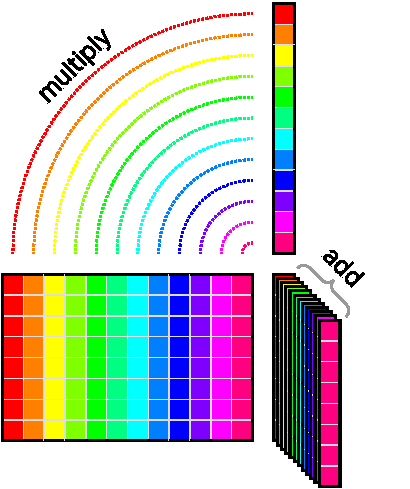
\includegraphics[width=5cm]{../assets/nnue/mv.pdf} }}%
\qquad
\subfloat[\centering Linear layer with sparse inputs]{{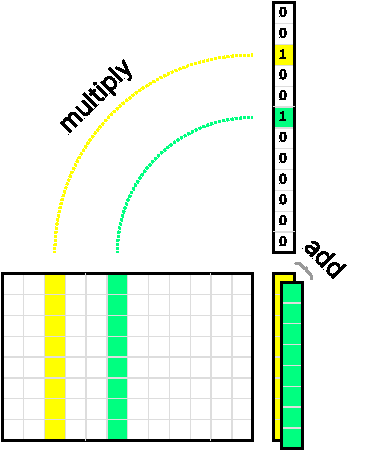
\includegraphics[width=5cm]{../assets/nnue/mvs.pdf} }}%
\caption{Linear layer operation comparison. Figures from \cite{nnue-pytorch}.}
\label{fig:linear_comparison}
\end{figure}

In the case of the first layer, the input is a very sparse one-hot encoded vector. This means that very few columns will have to be processed and the multiplication can be skipped altogether, due all inputs being either 0 or 1.

\paragraph[short]{Clipped ReLU} This is a simple activation that clips the output in the range $[0, 1]$. The operation is $\bm{y=\min(\max(x,0),1)}$.
The output of this activation function is the input for the next layer, and because of the aggresive quantization that will be described later, it is necessary to restrain the values so it does not overflow. \\

\subsection{Efficient updates}

When running a depth-first search algorithm, the state of the position is updated with every time time the algorithm \textit{makes} and \textit{unmakes} moves, usually before and after the recursion.
NNUEs are designed to work with this kind of search, since every time the algorithm \textit{makes} (or \textit{unmakes}) a move, the changes in the position are minimal (at most two pieces are affected), meaning that the amount of features becoming active or inactive is minimal as well. This is depicted in Figure \ref{fig:updates_tree}.

\begin{figure}[H]
\centering
\storechessboardstyle{3x3}{tinyboard,maxfield=c3,margin=false,showmover=false,hlabel=true,vlabel=true,pgfstyle=color,color=blue}
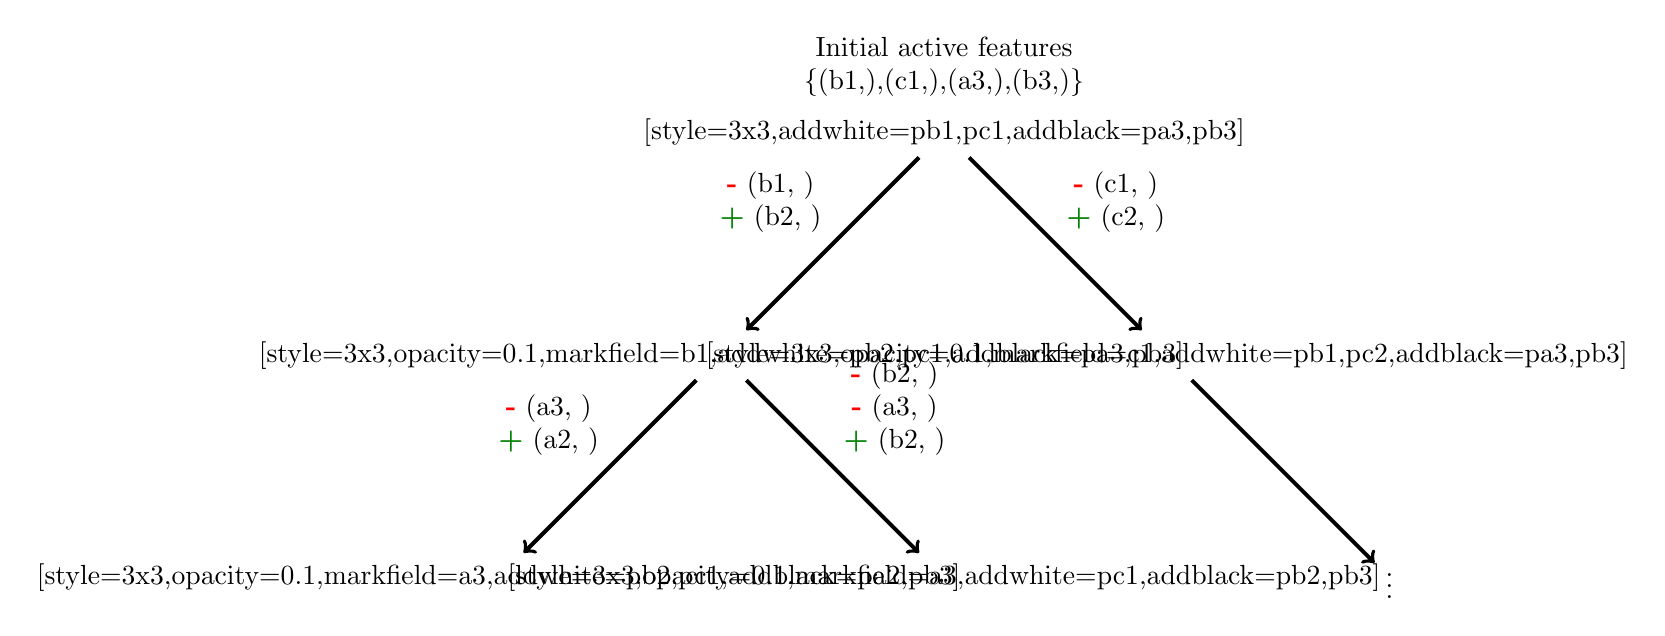
\begin{tikzpicture}[
    node distance=4cm,
    line width=0.5mm,
    auto
]

    \node[label={[align=center]Initial active features \\ \{(b1,\white),(c1,\white),(a3,\black),(b3,\black)\}}] (A) {\chessboard[style=3x3,addwhite={pb1,pc1},addblack={pa3,pb3}]};

    % childs of A
    \node (B) [below left of=A] {\chessboard[style=3x3,opacity=0.1,markfield={b1},addwhite={pb2,pc1},addblack={pa3,pb3}]};
    \node (C) [below right of=A] {\chessboard[style=3x3,opacity=0.1,markfield={c1},addwhite={pb1,pc2},addblack={pa3,pb3}]};

    % childs of B
    \node (D) [below left of=B] {\chessboard[style=3x3,opacity=0.1,markfield={a3},addwhite={pb2,pc1},addblack={pa2,pb3}]};
    \node (E) [below right of=B] {\chessboard[style=3x3,opacity=0.1,markfield={a3},addwhite={pc1},addblack={pb2,pb3}]};

    % childs of C
    \node (F) [below right of=C] {\vdots};

    % arrows of A
    \path[<-] (B) edge node[align=center] {\textbf{{\color{Red}-}} (b1, \white) \\ \textbf{{\color{Green}+}} (b2, \white)} (A);
    \path[->] (A) edge node[align=center] {\textbf{{\color{Red}-}} (c1, \white) \\ \textbf{{\color{Green}+}} (c2, \white)} (C);
    
    % arrows of B
    \path[<-] (D) edge node[align=center] {\textbf{{\color{Red}-}} (a3, \black) \\ \textbf{{\color{Green}+}} (a2, \black)} (B);
    \path[->] (B) edge node[align=center] {\textbf{{\color{Red}-}} (b2, \white) \\ \textbf{{\color{Red}-}} (a3, \black) \\ \textbf{{\color{Green}+}} (b2, \black)} (E);

    % arrows of C
    \path[<-] (F) edge node[align=center] {} (C);

\end{tikzpicture}
\caption{Partial tree of feature updates (\textcolor{Red}{removals} and \textcolor{Green}{additions}) for $\fs{SQUARE}_P \times \fs{COLOR}_P$ (white's point of view) in a simplified 3x3 pawn-only board.}
\label{fig:updates_tree}
\end{figure}

To take advantage of this during search, instead of computing all the features active in a position and then evaluate the network in its entirety, we can \textbf{accumulate} the output of the first linear layer and update it with when the position changes. Linear layers can be computed adding the corresponding columns of the weight matrix into the output, so when a feature becomes active or inactive, we can add or subtract the corresponding column to the output.


Recall that the way I defined feature sets, they always encode the position from white's position.


\subsection{Network}

arquitectura half, dos capas

pesada al principio y liviana al final, acumular filas de la primera capa en domove, undomove

\subsection{Quantization}

% https://github.com/official-stockfish/nnue-pytorch/blob/master/docs/nnue.md#quantization

The weights and operations in the neural network are in float domain. Floating point operations are too slow to achieve maximum performance, as it sacrifices too much speed. Quantizing the network to integer domain will inevitable introduce some error, but it far outweights the performance gain. In general, the deeper the network the more error is accumulated. Since NNUEs are very shallow by design, the error is negligible.

The objective is to take advantage of modern CPUs that allow doing low-precision integer arithmetic in parallel with 8, 16, 32 or even 64 8-bit integer values at a time. To achieve this, the best is to use the smallest integer type possible everywhere, to process more values at once. \\

[...]

\subsubsection{Stockfish quantization scheme}

In this thesis, I will use the same quantization scheme used in the engine Stockfish \cite{nnue-pytorch}. It uses int8 ($-128..127$) for inputs and weights, and int16 ($-32768..32767$) where int8 is not possible.
To convert the float values to integer, we need to multiply the weights and biases by some constant to translate them to a different range of values. Each layer is different, so I'll go through each one.

\begin{figure}[H]
\centering
\makebox[\textwidth]{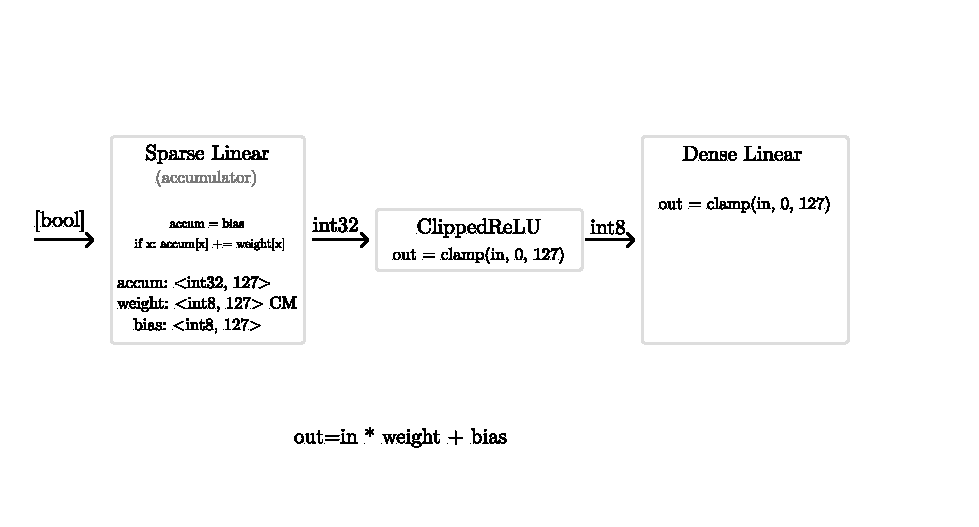
\includegraphics[width=\textwidth]{../assets/nnue/quantization.pdf}}
\caption{Simplified network showcasing all layers with quantization values}
\label{fig:quantization}
\end{figure}

\paragraph[short]{Input} Since we are using an accumualtor, there is not a real input to the model.

Inputs are quantized to 8 bits, so the range of values is $-128..127$. Since the inputs are hot encoded, the float values are 0.0 or 1.0, so the quantized values are either 0 or 127.

\paragraph[short]{Accumulator layer} The purpose of this layer is to accumulate rows of the first layer's weight matrix, which are values in 8 bits. Since the output of this layer will be the input for the next linear layer and it has the ClippedReLU activation, the output will also be in 8 bits.
But since we are accumulating 8 bits values and


and to output a clipped value of 8 bits for the next layer.

we can't accumulate using 8 bits since it would overflow.

COLUMN MAJOR

\paragraph[short]{Linear layer} no se tiene el mismo problema que en el accumulator layer porque la multiplicacion en SIMD se hace en 32 bits (osea sin hacer overflow), para despues aplicar clippedrelu a eso.

\paragraph[short]{ClippedReLU} Al estar cuantizado, el clipping pasa a ser de 0..1 a 0..127. El tamaño del input puede variar, 32 bits si viene del acumulador o 16 si viene de una capa intermedia, pero el resultado siempre está en 8 bits.

\textbf{Rango de activación}: en el modelo original usamos ClippedReLU, asi que queremos que el rango vaya de 0..1 a 0..127.


Siendo $\bm{x}$, $\bm{w}$ y $\bm{b}$ los parámetros de una capa lineal sin cuantizar e $\bm{y}$ la salida de la misma, se tiene que:

\begin{equation}
\begin{aligned}
\bm{y} &= \bm{x} \bm{w} + \bm{b} \\
s_a s_w \bm{y} &= (s_a \bm{x}) (s_w \bm{w}) + s_a s_w \bm{b} \\
\end{aligned}
\end{equation}



\vspace{1cm}
$s_o ((s_a \bm{x}) (s_w \bm{w}) + s_a s_w \bm{b}) = s_a s_w s_o \bm{y}$

. \\

The Stockfish repository provides a AVX2 implementation of the previous operations in C++. They have been ported to Rust for this thesis. The implementation was tested using the Pytorch model as reference (output match).

\subsection{Network sparsity}

o combinar con 3.2?
poner graficos con la sparsity de cada feature set, decir que es muy esparso todo y que se podría mejorar aún más

% Real effect of the factorizer :)

\section{Engine implementation}

:)

stockfish too complicated :)
\section{Training}

Given a feature set, the network architecture is completely defined, along with how to encode a position into its inputs. This section will describe two proposed methods to train the networks, each with its own loss function and training dataset.

\subsection{Source dataset}

Data is needed to train the network. The proposal for the thesis was to use the Lichess database \cite{lichessdb}, which provides a CC0 database with all the games ever played on the site, then score the positions using Stockfish. After some initial experiments, the networks were not performing as expected. Upon further reaserch, I found out that I was working with datasets too small for this task (order of hundreds of millions). I needed a larger dataset (order of \textbf{dozens of billions}), but it was impractical for me to generate it. Fortunately, I can use the same dataset that Stockfish uses to train its networks \cite{sf_nnue_dataset}, which should work well. Specifically, I went with the dataset used to train the first stage of the main network for Stockfish 16.1, which is 135GB of compressed \texttt{binpack} files. It was built by running Stockfish at 5000 nodes per move on multiple opening books\footnote{An opening book is a database of start positions (lines of play) generated with some criteria.}. Later stages use datasets generated by Leela Chess Zero (LC0), which is more expensive to compute but has higher quality evaluations.

The \texttt{binpack} format is a very efficient method of storing samples yet very complex to decode. Fortunately, Stockfish provides a tool to export this data into a text representation. I had to modify it to export it in the format I wanted. I changed the \texttt{emitPlainEntry} function in \texttt{nnue\_data\_binpack\_format.h} to the code in Appendix \ref{appendix:emitPlainEntry}. The resulting file was 2.59 terabytes in size and contained \textbf{48.4 billion samples}. There is one sample per line with the format:

\begin{center}
\begin{tabular}{|cp{0.0005cm}cp{0.0005cm}c|}
\hline
\textbf{FEN\footnotemark} & , & \textbf{Score} & , & \textbf{Best move} \\
\hline
\end{tabular}
\end{center}

\footnotetext{Standard notation to describe positions of a chess game. It is a sequence of ASCII characters.}

The file was too big to be practical, and it would wear off my SSD, so I made a tool to compact the data into a similar format. The new format exploits the fact that samples in a row belong to the same game. This means that contiguous FENs are a move from a previous one, so it stores the move instead of the FEN:

\begin{center}
\begin{tabular}{|cp{0.0005cm}cp{0.0005cm}c|}
\hline
\textbf{FEN} & , & \textbf{Score} & , & \textbf{Best move} \\
\hline
\end{tabular}
(
\begin{tabular}{|p{0.0005cm}cp{0.0005cm}cp{0.0005cm}c|}
\hline
, & \textbf{Actual move} & , & \textbf{Score} & , & \textbf{Best move} \\
\hline
\end{tabular}
) *\footnote{Repeated zero or more times.}
\end{center}

As you can see, the new format is compatible with the last one, so only one reader was implemented. After compacting the data, the file went down to a manageable 522 gigabytes. Also, reading a single FEN and later applying moves to it is much faster than parsing a FEN every time. \\

There are many positions in the dataset that are known to not be good for training. Remember that the engine is doing quiescent search, so it does a smaller search looking for quiet positions to evaluate. This means that positions where the \enquote{best} move is a capture, or there is a check, are filtered out when building the training batch. \\

Each training method will generate a new derived dataset based on these samples.

% Lichess is a free online site to play chess, and thankfully it provides a CC0 database \cite{lichessdb} with all the games ever played on the site. It consists of serveral compressed PGN files\footnote{Portable Game Notation: a textual format to store chess games (moves and metadata)} splitted by month since 2013, that add up to $1.71$TB compressed. The whole database contains over 5.5 billion games, that equates to around 200 billion positions. In practice, that many positions are too much to handle so I'll use only a fraction of them and take only one sample per game to increase the diversity of positions.

% The Lichess database also provides a database of puzzles
% hablar de esto en otro lado (results? eval?)

% A single game can have lots of positions, most of which are shared with millions of other games, mostly during the early game. This is a problem of its own: trying to sample positions from a game with a suitable distribution. In this work, I have chosen to only consider positions 20 half-moves into the game.

\subsection{Method 1: Score target}

The main method to train the network will use the scores provided in the dataset as targets. I expect the networks to learn to predict the evaluation of a position as Stockfish would do.

\setcounter{secnumdepth}{4}
\subsubsection{Score-space to WDL-space}

Evaluations in the dataset are values ranging from -10000 to 10000. We call this range of values the score-space, also referred to as the \textit{centipawn scale} (or something proportional to it). We want the network to output the same values as the dataset, in \textit{score-space}.

The WDL-space is a different scale in [0, 1] where 0 is a loss, 0.5 is a draw, and 1 is a win. The WDL (win-draw-loss) model \cite{wdl-model} states that the win rate for a position can be modeled as a function of the evaluation of the position. The data shows that the logistic function (sigmoid) gives a good approximation for the evaluation $f(P)$:

\[
\mathcal{W}(f(P)) = \sigma\left(\frac{f(P)-a}{b}\right) = \frac{1}{1 + e^{-\frac{f(P)-a}{b}}}
\]

where $a$ and $b$ need to be fitted to the data. The value of $a$ is the evaluation where a 50\% winrate is observed, and $b$ indicates how fast the winrate changes when the evaluation change. The fitted sigmoid is shown in figure \ref{wdl-fit}, and the values obtained are $a=1.28$ and $b=297.21$.

\begin{figure}[H]
\centering
\makebox[\textwidth]{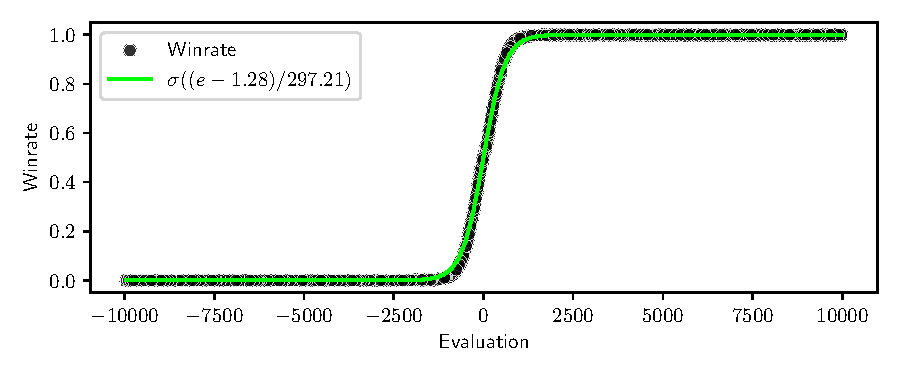
\includegraphics[width=\textwidth]{../assets/sigmoid_fit.pdf}}
\caption{WDL model function (sigmoid) fitted to 100 million evaluations in the dataset.}
\label{wdl-fit}
\end{figure}


During training, it is better to use a loss function with the target and output of the model in WDL-space instead of score-space. WDL-space has some advantages over score-space:

\begin{itemize}
\item Large evaluations are \enquote{closer} together in WDL-space, since having a score of 7500 or 8000 is not that different in terms of winrate (less than 1\%) than between 50 and 550 (more than 30\%). This is desirable because the evaluations do not need to be that precise when the outcome of the game is almost decided.
\item The result of a game can be interpolated in WDL-space. If we introduce a new parameter $\lambda$, we can interpolate the evaluation $f(P)$ and the game result $r$ (in WDL-space) using: $\lambda \cdot \mathcal{W}(f(P)) + (1 - \lambda) \cdot r$. This way, the information about the outcome of the game can be used to steer the network in the right direction. This is not implemented in this work.
\item Values in WDL-space are smaller than in score-space, so it avoids large gradients.
\end{itemize}




\subsubsection{Loss function}

The loss function chosen is mean squared error (MSE) with a power of 2.6 (the value used by the Stockfish's official trainer) given by

% q = (output / out_scaling).sigmoid()
% p = (target / in_scaling).sigmoid()
% loss = torch.pow(torch.abs(p - q), 2.6).mean()

\[
\mathcal{L}(y,f(x,\bm{W}))= \frac{1}{N} \sum_i^N \left| \mathcal{W}(y_i) - \mathcal{W}(f(x_i,\bm{W})) \right| ^{2.6}
\]

where\dots

\begin{enumerate}
\itemsep0em
\item $N$ is the number of samples.
\item $y$ are the target scores.
\item $f$ is the model.
\item $x$ are the inputs (encoded feature sets).
\item $\bm{W}$ are the parameters of the model.
\item $\mathcal{W}$ is the winrate function that maps from score-space to WDL-space.
\end{enumerate}

\subsection{Method 2: PQR triplets}

This is an additional technique I wanted to try, described in \cite{dlchess:2014}. The method is based on the assumption that moves in the training data are better than random. In the blog they used human moves from the Lichess database \cite{lichessdb}, so they rely on the fact that humans make good or near-optimal moves most of the time, even if they are amateurs. In my case, I will use Stockfish moves, which are extremely good. This method does not use the scores provided; it will have to learn them from scratch. Of course this is way harder to train, but I'm curious to see how far the following idea can go.

Remember that we are trying to obtain a function $f$ (the model) to give an evaluation of a position. The idea is based on the following two principles:

\begin{enumerate}
\item For two positions in succession $P \rightarrow Q$ observed in a game, we will have \mbox{$f(P)=-f(Q)$}. This comes from the fact that the game is zero-sum.
\item Going from the position $P$, not to the observed position $Q$, but to a \textit{random} position $P \rightarrow R$, we must have $f(R) > f(Q)$ because the random move is better for the next player and worse for the player that made the move.
\end{enumerate}

If these reasonable assumptions hold, a loss function that expresses the equality in (1) and the inequality in (2) can be constructed.

% Consider an optimal $f$, that outputs $-1,0,1$ depending on who wins.
% With infinite compute, $f$ would be the result of running minimax to the end of the game, since minimax always finds optimal moves.

\subsubsection{Loss function}

The loss function is the sum of the negative log-likelihood of the inequalities: ${f(R) > f(Q)}$, ${f(P) > - f(Q)}$ and ${f(P) < -f(Q)}$. The last two are a way to express the equality \mbox{$f(P)=-f(Q)$}. Each term is the negative log-likelihood function of the known Bradley-Terry model \cite{bradley-terry:1952}, that models the probability of an item (in our case a position) \enquote{beating} another item.

The loss function is given by

\begin{align*}
\mathcal{L}(x^P, x^Q, x^R, \bm{W})=
\frac{1}{N}
\sum_i^N
& -\log\left(\sigma(r_i - q_i)\right) \\
& -\log\left(\sigma(p_i + q_i)\right) \\
& -\log\left(\sigma(-(p_i + q_i))\right)
\end{align*}

where\dots

\begin{enumerate}
\itemsep0em
\item $N$ is the number of samples.
\item $x^i$ are the inputs (encoded feature sets) for the $i \in \{P,Q,R\}$ positions.
\item $f$ is the model.
\item $\bm{W}$ are the parameters of the model.
\item $\mathcal{W}$ is the winrate function that maps from score-space to WDL-space.
\item $\overline{\mathcal{W}}(x) = 2 \mathcal{W}(x) - 1$ is a function that maps from WDL-space [0, 1] to $[-1, 1]$, so that $\overline{\mathcal{W}}(x) = -\overline{\mathcal{W}}(-x)$.
\item $
p_i = \overline{\mathcal{W}}(f(x^P_i, \bm{W})),\text{ }
q_i = \overline{\mathcal{W}}(f(x^Q_i, \bm{W}),\text{ }
r_i = \overline{\mathcal{W}}(f(x^R_i, \bm{W})
$. Note that quantization is happening in this method too, so the output of the model is being scaled appropriately.
\end{enumerate}



Let's break down the loss function in a more intuitive way. We want the loss function to be small when the model is generating the correct evaluations and large when it is not. Let's look at the graph of the function $-\log(\sigma(x))$:

\begin{figure}[H]
\centering
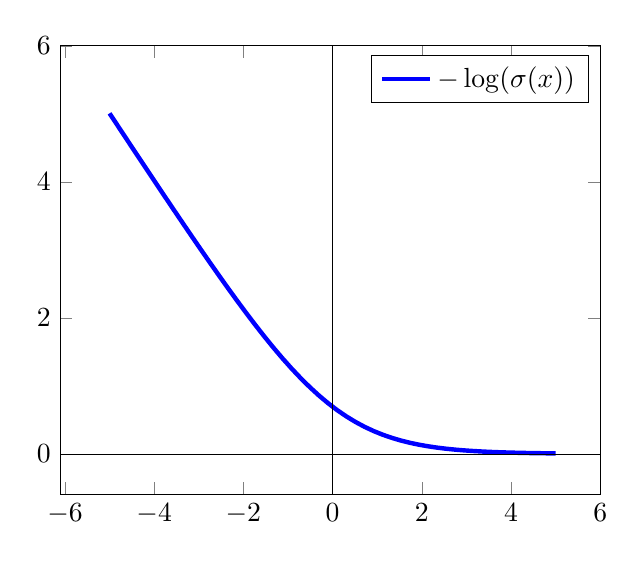
\begin{tikzpicture}
\begin{axis}[xmax=6,ymax=6, samples=50]
\addplot[blue, ultra thick] (x,{-ln(1/(1+e^-x))});
\draw[ultra thin] (axis cs:\pgfkeysvalueof{/pgfplots/xmin},0) -- (axis cs:\pgfkeysvalueof{/pgfplots/xmax},0);
\draw[ultra thin] (axis cs:0,\pgfkeysvalueof{/pgfplots/ymin}) -- (axis cs:0,\pgfkeysvalueof{/pgfplots/ymax});
\addlegendentry{$-\log(\sigma(x))$}
\end{axis}
\end{tikzpicture}
\end{figure}

The function approaches 0 when $x$ grows and approaches $\infty$ when $x$ goes to $-\infty$.

Let's look at each of the terms:

\begin{enumerate}
\itemsep0em
\item $-\log(\sigma(r_i - q_i))$: This term is small when $r_i > q_i$, and large when $r_i < q_i$.
\item $-\log(\sigma(p_i + q_i))$: This term is small when $p_i > -q_i$, and large when $p_i < -q_i$.
\item $-\log(\sigma(-(p_i + q_i))$: This term is small when $p_i < -q_i$, and large when $p_i > -q_i$.
\end{enumerate}

The term (1) holds the inequality $f(R) > f(Q)$, and the terms (2) and (3) hold the equality $f(P) = -f(Q)$. The loss function is the sum of the three terms, so the model is encouraged when it satisfies the inequalities and penalized when it does not.

\subsection{Setup}


The project is written in two languages: Rust and Python. The Rust part is used to process dataset files, generate statistics, and provide final training batches for Python to consume. The Python part defines the Pytorch model, runs the training loop, quantizes the model, and runs the evaluations. \\

The training process is started by running a Python script (\texttt{scrips/train.py}) and it requires to define the model architecture (number of neurons on each layer), general training parameters (learning rate, batch size, epochs, checkpoints, etc.) and the feature set to use, which in turn determines the size of the batches. For example, if PQR is used, the size of a sample is three times the size of the feature set times two (because it is siamese), and if it is score target, it is the size of the feature set times two plus one for the target score.

To orchestrate training runs, the platform Weights and Biases (WandB) is used. It provides automatic sweeping of hyperparameters, logging of metrics, and visualizations. Results are exported from the platform in CSV and then processed by Python scripts. \\

The training data has to be converted to an actual tensor of floats to be consumed by Pytorch. This is done by a Rust subprocess running the subcommand \texttt{batch-loader} that reads the training data file and generates training batches for the specified feature set in a shared memory buffer.

The batch generation process is heavily parallelized. Let's call $N$ the number of threads ($N=8$ was used). When the process starts, it splits the dataset file into $N$ equal parts and assigns each part to a thread. Each thread reads samples sequentially and builds the batch in a buffer. The buffer is then sent to the main thread, where it is copied to the shared memory buffer.

The Python script copies the data from the shared buffer at the start of each iteration, allowing Rust to generate the next batch (in the CPU) while Pytorch is training the current batch (in the GPU). To coordinate the memory access between the two processes, a single byte is sent using standard I/O. The sequence of a training loop is shown in figure \ref{training-loop}.

\begin{figure}[H]
\centering
\makebox[\textwidth]{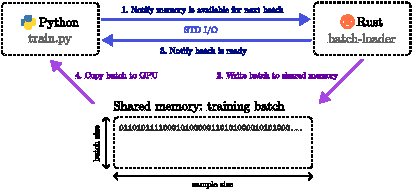
\includegraphics[width=\textwidth]{../assets/training-loop.pdf}}
\caption{Sequence of steps to send a batch from the \texttt{batch-loader} subprocess in Rust to Pytorch.}
\label{training-loop}
\end{figure}

Given that the input vector is multiple-hot encoded, the data written by the Rust process are not float values. Instead, they are 64-bit integers acting as a bitset. Before passing the vector to the model, it is expanded into floats. This means 64 floats can be packed into a single 64-bit integer, meaning a \textbf{96.875\%} reduction in memory usage (from 256 to 8 bytes). The speedup obtained by this optimization was substantial. The compression can be further improved using sparse tensors, but it is not implemented in this work. \\

%\begin{figure}[H]
%\centering
%\makebox[\textwidth]{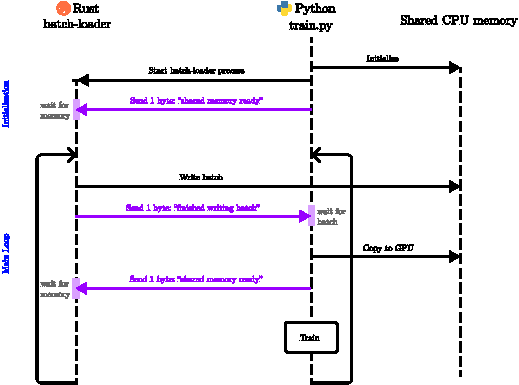
\includegraphics[width=\textwidth]{../%assets/training.pdf}}
%\caption{assad.}
%\end{figure}

% [evaluation?]
% [a esta seccion se le pueden agregar mil cosas]
% [multithreaded, perf]
% decir que en "All" tengo 450 it/s (7.3M pos/sec)



\section{Results}

hablar del tradeoff de los feature sets, la primera capa, y demás

vertical and horizontal data, probar dataset sin info vertical u horizonal / ambos y ver que pasa
ver si agregar capas posteriores ayuda o no "layer layers small increase in perf"

measure updates per move average and refreshes average per FS



\subsection{Active neurons}

medir si hay feature sets que no usen neuronas, que esto disparo el uso de HalfTopK

average number of features enabled by feature set (cantidad y porcentaje)



future work: triplet loss?

\section{Final words}
\subsection{Conclusions}
\subsection{Future work}


% prunning feature sets? quizas no ayuda, solo para training, no se. ver bien

% lo ideal de un feature set son patrones que NO se den en simultáneo? asi podes aprender mas usando menos neuronas

future work: hacer que no sea uniforme el sampling de las posiciones para armar los datasets

future work: triplet loss?

deduplication de posiciones (al computar el score de Stockfish)

maybe implementing a custom engine was not a good idea. bugs and stuff


\newpage
\printbibliography

\end{document}


% orden de escritura:
% encodings
% training
% results
% el resto...

% https://ctan.dcc.uchile.cl/info/symbols/comprehensive/symbols-a4.pdf